
\documentclass[12pt]{amsart}
\usepackage{geometry} % see geometry.pdf on how to lay out the page. There's lots.
\geometry{a4paper} % or letter or a5paper or ... etc
% \geometry{landscape} % rotated page geometry
\usepackage{graphicx} %插入图片的宏包
\usepackage{float} %设置图片浮动位置的宏包
\usepackage{subfigure} %插入多图时用子图显示的宏包

% See the ``Article customise'' template for come common customisations

\title{}
\author{}
\date{} % delete this line to display the current date

%%% BEGIN DOCUMENT
\begin{document}

\section{Original Design}

\begin{figure}[H] %H为当前位置,!htb为忽略美学标准,htbp为浮动图形
\centering %图片居中
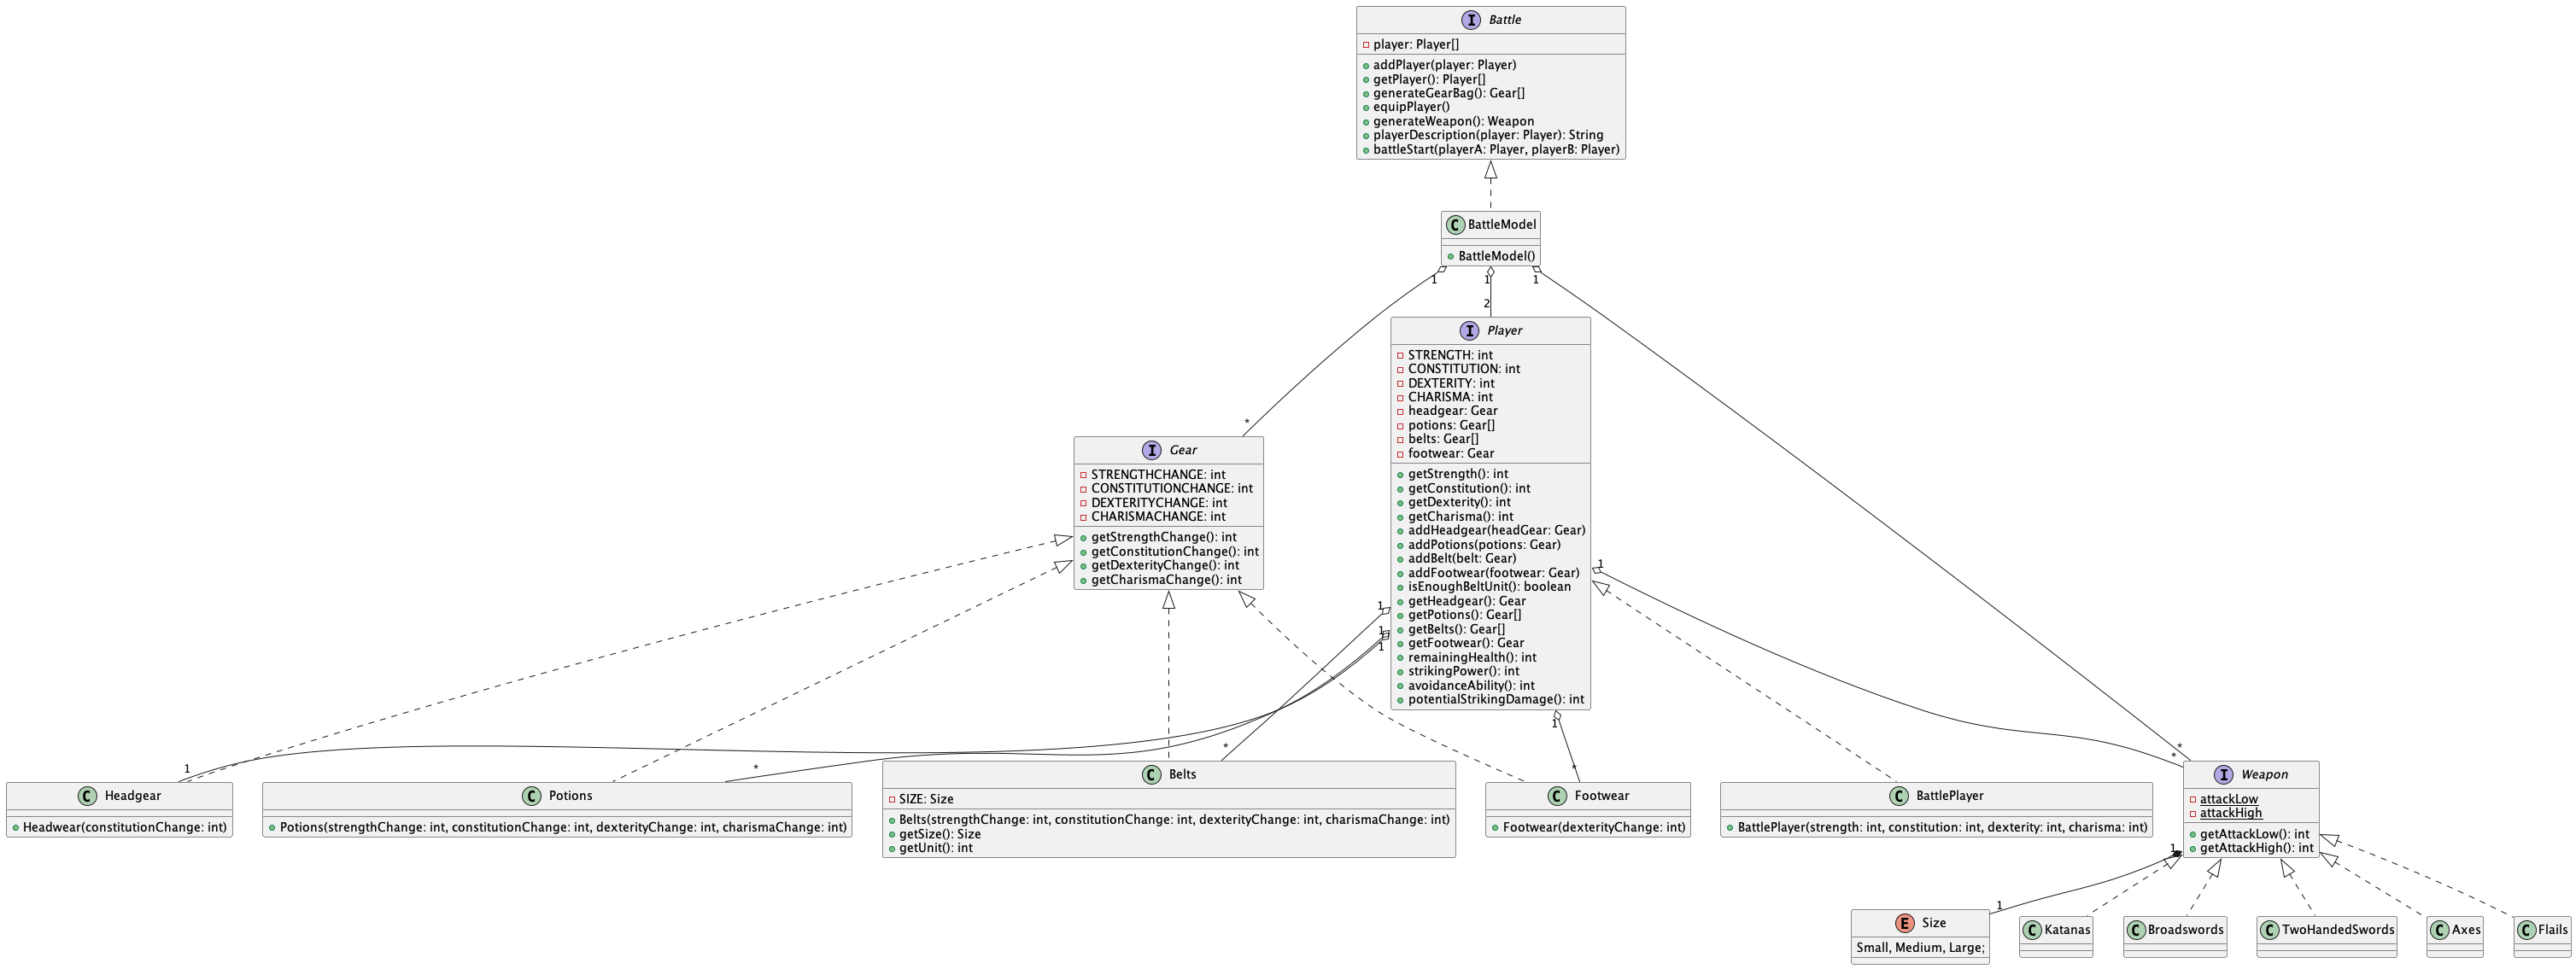
\includegraphics[width=2\textwidth, angle=90]{uml.png} %插入图片,[]中设置图片大小,{}中是图片文件名
\end{figure}

\newpage

\section{BattlePlayer}

\begin{table}[htbp]
   %\topcaption{Table captions are better up top} % requires the topcapt package
   \begin{tabular}{@{} lcr @{}} % Column formatting, @{} suppresses leading/trailing space

      Method      & Input & Expected \\
         Constructor with invalid values       & BattlePlayer(0, 0, 0, 0)     &  IllegalArgumentException \\
         Constructor with valid values       & BattlePlayer(2, 2, 2, 2)      &   \\
         test remainHealth       & remainHealth()      &   \\
         test strikingPower       & strikingPower()      &   \\
         test avoidanceAbility       & avoidanceAbility()      &   \\
         test potentialStrikingDamage       & potentialStrikingDamage()      &   \\
    \end{tabular}
\end{table}

%\newpage

\section{Headgear}

\begin{table}[htbp]
   %\topcaption{Table captions are better up top} % requires the topcapt package
   \begin{tabular}{@{} lcr @{}} % Column formatting, @{} suppresses leading/trailing space

      Method      & Input & Expected \\
         Constructor with valid values       & Headgear(2)      &   \\
    \end{tabular}
\end{table}

\section{Potions}

\begin{table}[htbp]
   %\topcaption{Table captions are better up top} % requires the topcapt package
   \begin{tabular}{@{} lcr @{}} % Column formatting, @{} suppresses leading/trailing space

      Method      & Input & Expected \\
         Constructor with invalid values       & Potions(2, 2, 2, 2)     &  IllegalArgumentException \\
         Constructor with valid values       & Potions(2, 0, 0,0)      &   \\
    \end{tabular}
\end{table}

\section{Footwear}

\begin{table}[htbp]
   %\topcaption{Table captions are better up top} % requires the topcapt package
   \begin{tabular}{@{} lcr @{}} % Column formatting, @{} suppresses leading/trailing space

      Method      & Input & Expected \\
         Constructor with valid values       & Footwear(2)     &   \\
    \end{tabular}
\end{table}

\section{BattleModel}

\begin{table}[htbp]
   %\topcaption{Table captions are better up top} % requires the topcapt package
   \begin{tabular}{@{} lcr @{}} % Column formatting, @{} suppresses leading/trailing space

      Method      & Input & Expected \\
         Constructor      & BattleModel()    &   \\
    \end{tabular}
\end{table}

\newpage

\section{Final Design}
\begin{figure}[H] %H为当前位置,!htb为忽略美学标准,htbp为浮动图形
\centering %图片居中
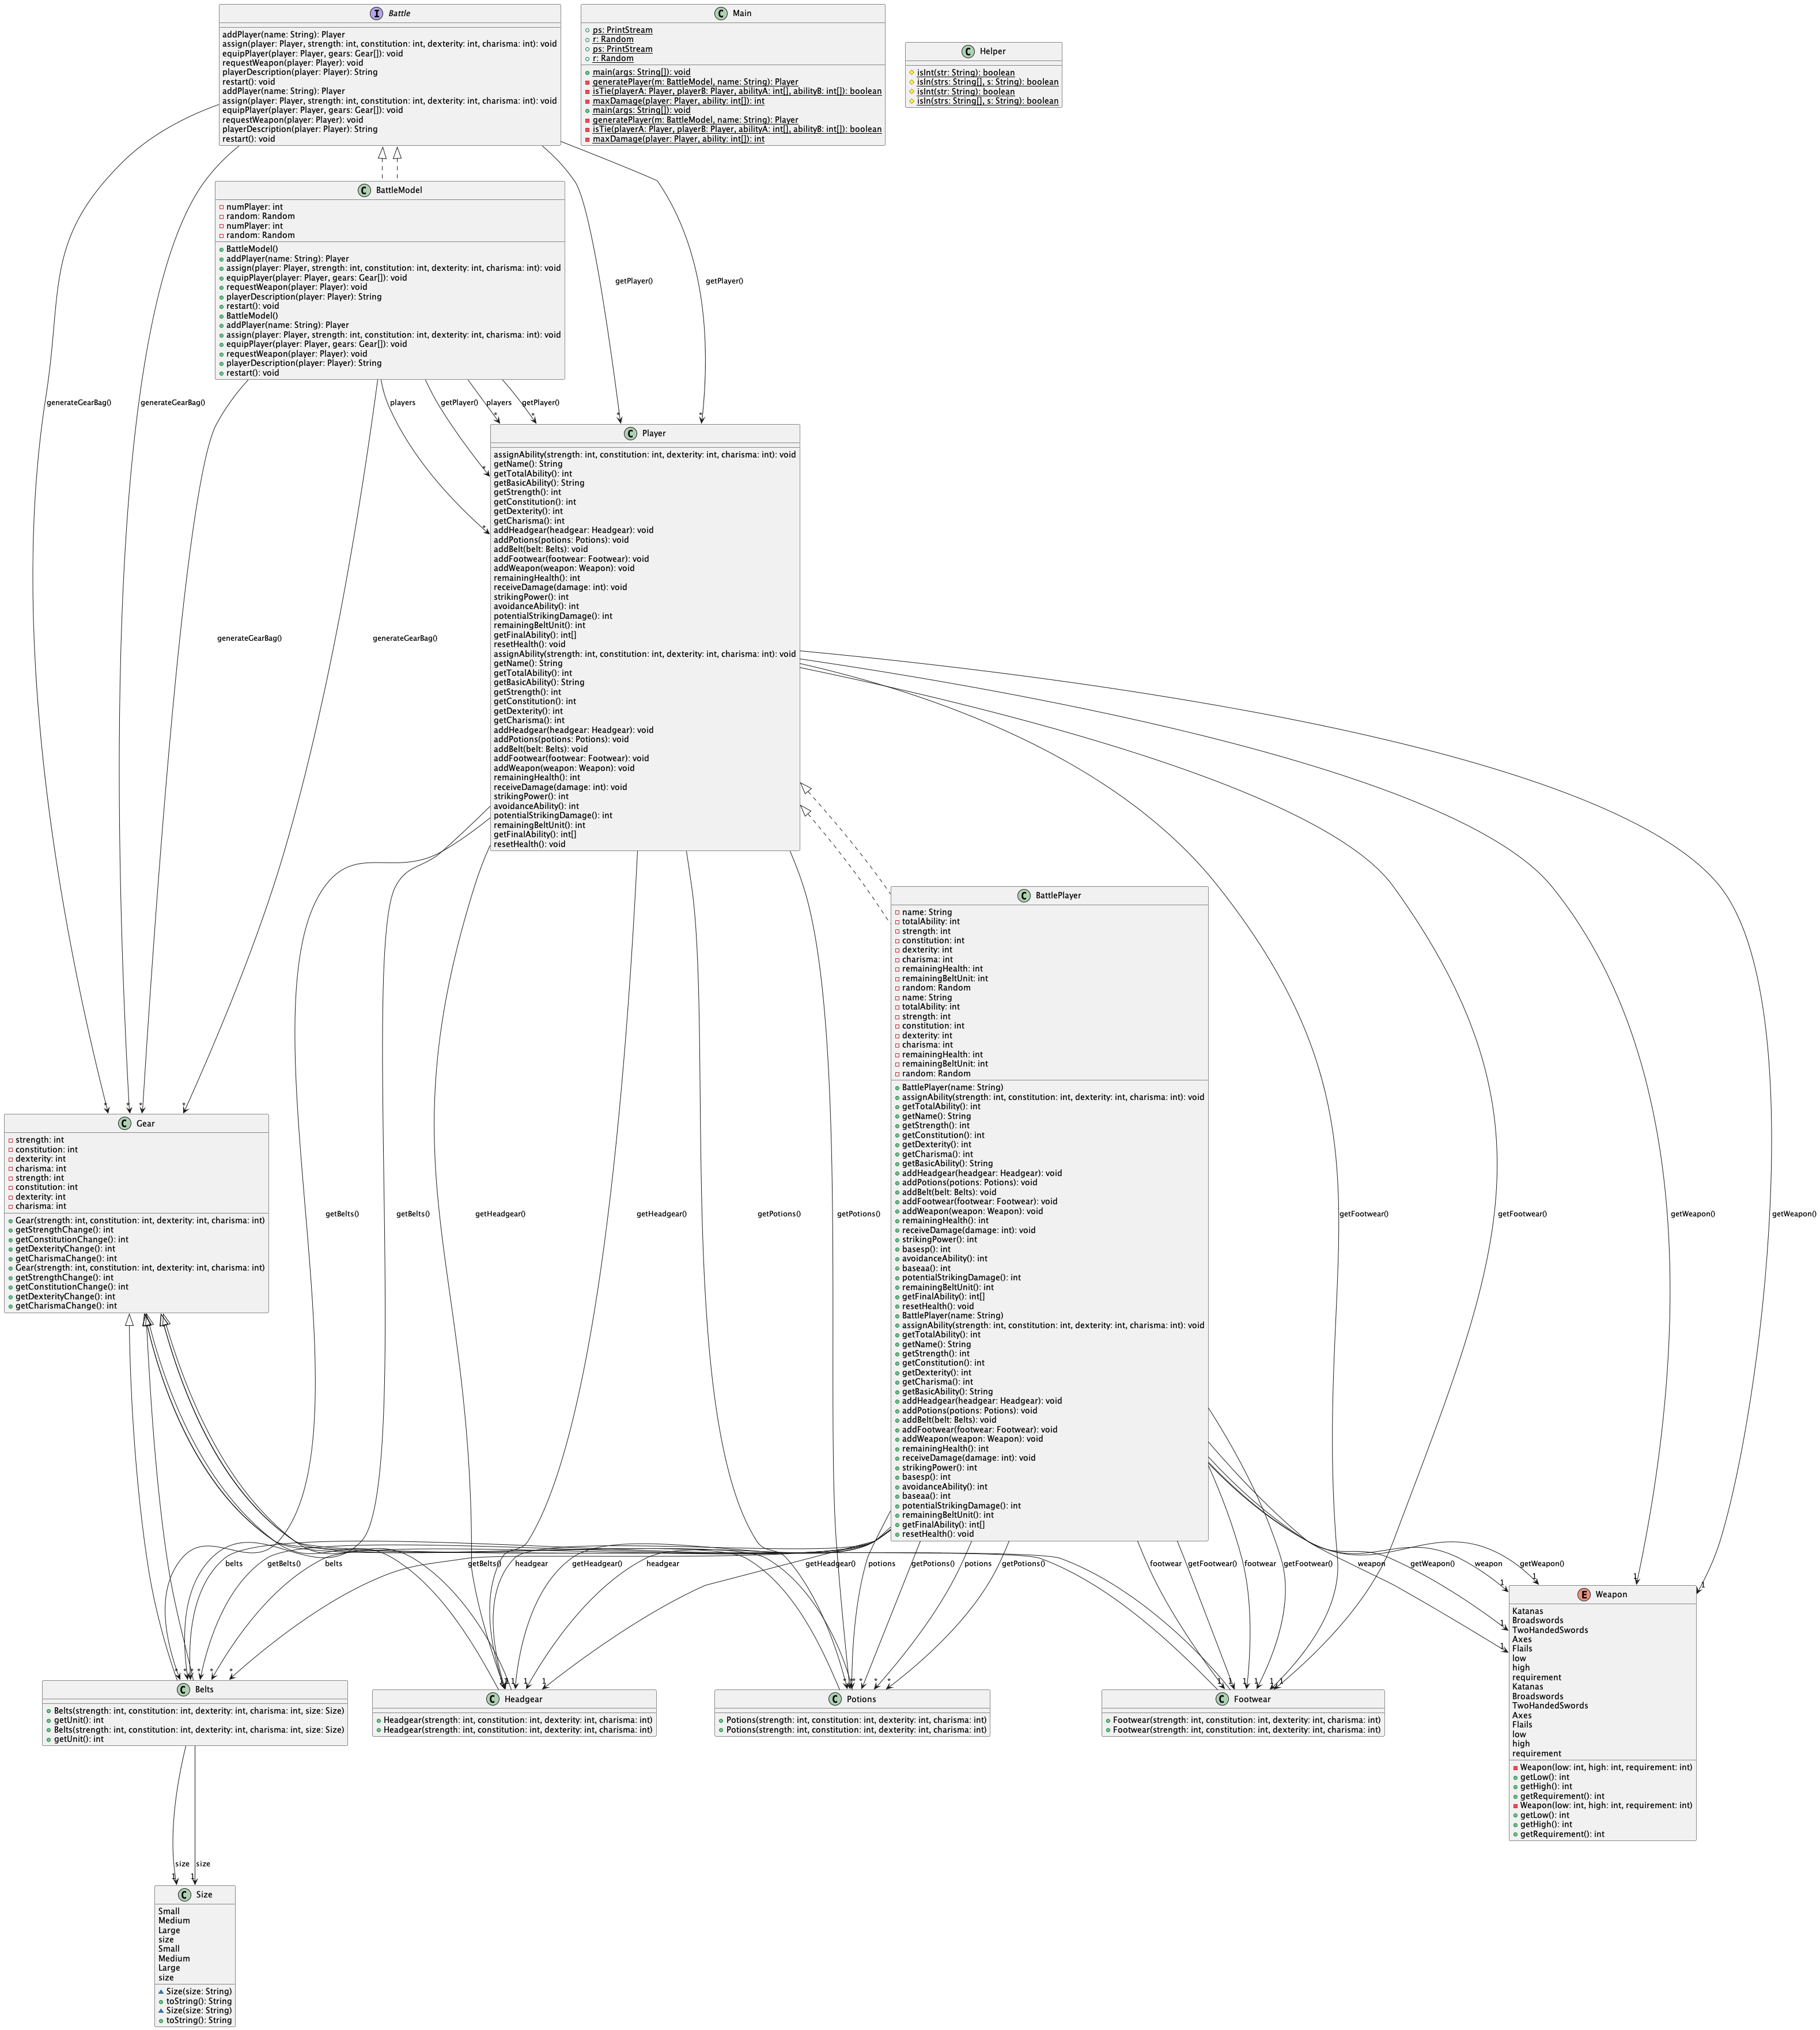
\includegraphics[width=1.2\textwidth,]{uml_final.png} %插入图片,[]中设置图片大小,{}中是图片文件名
\end{figure}

\newpage

\section{GearTest}

\begin{table}[htbp]
   %\topcaption{Table captions are better up top} % requires the topcapt package
   \begin{tabular}{@{} lcr @{}} % Column formatting, @{} suppresses leading/trailing space

      Method      & Input & Expected \\
         Constructor of a gear       & strength of the gear     &  equal \\
         Constructor of a gear       & constitution of the gear     &  equal \\
         Constructor of a gear       & dexterity of the gear     &  equal \\
         Constructor of a gear       & charisma of the gear     &  equal \\
         Constructor of a gear       & size of the belt     &  equal \\
    \end{tabular}
\end{table}

\section{WeaponTest}

\begin{table}[htbp]
   %\topcaption{Table captions are better up top} % requires the topcapt package
   \begin{tabular}{@{} lcr @{}} % Column formatting, @{} suppresses leading/trailing space

      Method      & Input & Expected \\
         Constructor of a weapon       & low attack range of the weapon     &  equal \\
         Constructor of a weapon       & high attack range of the weapon      &  equal \\

    \end{tabular}
\end{table}


\section{BattleTest}
\begin{table}[htbp]
   %\topcaption{Table captions are better up top} % requires the topcapt package
   \begin{tabular}{@{} lcr @{}} % Column formatting, @{} suppresses leading/trailing space

      Method      & Input & Expected \\
         Non-positive ability of a player       & 0 charisma     &  IllegalArgumentException \\
         Adding gear doesn't change base ability       & base constitution and constitution after adding headgear     &  equal \\
         Correct total health & assertEquals(total, player.remainingHealth()) & pass \\
         Correct striking power & assertEquals(total - 3, ((BattlePlayer) player).basesp()) & pass \\
         Correct avoidance & assertEquals(1, ((BattlePlayer) player).baseaa()) & pass \\
         Correct potential damage & assertEquals(total - 3, player.potentialStrikingDamage()) & pass \\
         Negative damage change nothing & do -1 damage and check if change remain health & don't change\\
         Correct updating health after damage & do 1 damage and check & correct change \\
         Test entering arena with bare hand & check no gear and no weapon & pass \\
         Test one headgear & add two headgear & the last headgear is stored \\
         Test one footwear & add two footwear & the last footwear is stored \\
         Test belt unit & add 2 large belt and 1 medium belt & successfully added \\
         

    \end{tabular}
\end{table}


\end{document}